\chapter{Complete Test Results}\label{appaB}
This appendix shows the complete result tables.
They are not in chapter \ref{EmChap} for clarity.
The detailed metrics for the single datasets can be looked up here.
Furthermore, in this chapter there are test results which have not been showed yet. 
The reason for this is that the test in his construction has no cross-validation.
However, this test is sometimes used to test transfer learning classification \cite{Long.} and can be found in section \ref{BSecCom}.
The complete five two cross-validation test results are shown in section \ref{BSecFT}.

\section{Five Two Comparison}\label{BSecFT}
This section shows the detailed metrics of the cross-validation test.
The table is showing the mean over the 5x2 cv F test, which is a total of ten repetitions.
Every repetition has it's unique sampling from the dataset. 
Note that in table \ref{BTableFTErr} shows not only the mean but the standard deviation in brackets.
This result is also plotted in figure \ref{FigErrorImgDatasetsB} for images and plotted in figure \ref{FigErrorReutersDatasetsB} for Reuters.
The number of a dataset is the order of the sets, shown, for example, in \ref{BTableFTErr}.
Furthermore, in table \ref{BTableFTAUC}, the \acs{AUC} values are shown. 
The used mean number of support vectors can be viewed in table \ref{BTableFTNev}.
The last table \ref{BTableFTTime} shows the needed time in seconds.  
\begin{table}[]
	\centering
	\resizebox{\textwidth}{!}{%
		\begin{tabular}{@{}ccccccccc@{}}
			\toprule
			\textbf{Error Image}   & SVM            & PCVM  & PCTKVM\textsubscript{$\theta$Est} & PCTKVM & TCA            & JDA   & GFK   & TKL            \\ \midrule
			C vs A                 & \textbf{52.38} (2.30)& 61.77 (2.04)& 57.12 (2.78)& 57.35  (2.88)& 53.11          (3.28)& 53.32 (3.00)& 63.68 (3.49)& 53.70 (1.72)          \\
			C vs D                 & 57.45 (5.03)	& 64.33 (5.19)& 60.24 (6.23)&\textbf{ 56.69 } (5.05)& 63.44          (4.45)& 58.72 (4.31)& 65.21 (4.94)& 57.71  (4.21)        \\
			C vs W                 & 66.70          (4.25)& 71.46 (4.21)& 65.44 (5.6)& 63.72  (6.57)& 70.30          (5.11)& 64.76 (6.34)& 73.22 (2.27)& \textbf{63.52}(2.35) \\
			A vs C                 & 59.54          (2.61)& 65.24 (2.14)& 62.42 (2.74)& 61.91  (2.27)& 58.66          (2.12)& 58.90 (1.33)& 66.20 (1.44)& \textbf{58.70}(2.21) \\
			A vs D                 & 66.90          (4.86)& 70.86 (5.71)& 65.72 (3.12)& 63.82  (4.09)& 64.33          (4.34)& 62.33 (6.85)& 72.25 (4.08)& \textbf{60.90} (5.10)\\
			A vs W                 & 69.51          (1.91)& 70.91 (2.59)& 67.86 (4.34)& 66.67  (5.05)& 69.44          (4.25)& 67.34 (2.42)& 76.01 (2.07)& \textbf{64.29} (2.94)\\
			D vs C                 & 75.41          (1.13)& 78.15 (2.05)& 72.08 (2.39)& 74.07  (3.09)& 71.83          (1.78)& 72.38 (2.04)& 72.47 (2.38)& \textbf{70.94} (2.52)\\
			D vs A                 & 73.63          (1.61)& 77.06 (2.52)& 72.44 (2.07)& 74.03  (2.47)& \textbf{68.93} (2.97)& 66.99 (2.68)& 71.25 (2.34)& 70.39 (2.73)          \\
			D vs W                 & 45.77          (2.97)& 64.54 (5.35)& 47.27 (5.57)& 47.46  (4.74)& 32.81          (3.87)& 36.07 (2.84)& 36.34 (4.83)& \textbf{32.47}(4.55) \\
			W vs C                 & 73.86          (1.52)& 76.49 (1.76)& 73.70 (2.1)& 74.14  (2.79)& \textbf{68.44} (1.63)& 74.07 (1.63)& 74.64 (1.39)& 68.51         (1.81) \\
			W vs A                 & 71.84          (1.24)& 73.07 (1.69)& 70.35 (1.83)& 71.07  (2.92)& \textbf{66.28} (1.53)& 72.13 (1.55)& 71.27 (2.24)& 68.08      (1.45)    \\
			W vs D                 & \textbf{25.10} (3.60)& 43.69 (4.96)& 47.01 (3.07)& 40.76  (3.04)& 27.13          (4.61)& 25.61 (3.83)& 28.29 (4.01)& 29.81   (5.20)       \\\midrule
			RSME                   & 61.59          (14.71)& 68.23 (9.35)& 63.64 (9.15)& 62.76  (14.81)& 59.67          (15.39)& 59.50 (13.63)& 64.33 (6.88)& \textbf{10.65} \\\midrule
			\textbf{Error Reuters} & SVM            & PCVM  & PCTKVM\textsubscript{$\theta$Est} & PCTKVM & TCA            & JDA   & GFK   & TKL            \\
			Orgs vs People         & 23.01          (1.58)& 26.77 (3.18)& 20.65(1.93)& 20.45  (1.95)& 22.78          (3.14)& 24.88 (2.61)& 26.95 (2.65)& \textbf{19.29} (1.73)\\
			People vs Orgs         & 21.07          (1.72)& 27.77 (2.19)& 15.94(1.96)& 14.05  (8.68)& 19.68          (2.00)& 23.23 (1.93)& 28.23 (2.46)& \textbf{12.76} (1.16)\\
			Orgs vs Places         & 30.62          (2.22)& 33.42 (6.10)& 30.82 (11.08)& 23.78  (2.26)& 28.38          (3.00)& 28.30 (1.51)& 33.46 (1.83)& \textbf{22.84} (1.62)\\
			Places vs Orgs         & 35.45          (2.24)& 35.49 (8.19)& 36.14 (7.38)& 27.62  (2.66)& 32.42          (3.91)& 35.37 (4.39)& 35.73 (2.69)& \textbf{18.33} (3.75)\\
			Places vs People       & 39.68          (2.35)& 41.01 (6.98)& 33.96 (9.29)& 29.71  (5.03)& 40.58          (4.11)& 42.41 (2.59)& 40.24 (4.37)& \textbf{29.55} (1.46)\\
			People vs Places       & 41.08          (1.98)& 40.69 (5.52)& 33.96 (8.17)& 41.08  (1.33)& 41.39          (3.26)& 43.51 (2.23)& 42.56 (2.46)& \textbf{33.42} (3.28)\\\midrule
			RSME                   & 31.88          (8.43)& 34.48 (5.93)&  30.78 (10.35)& 26.28  (9.32)& 31.03          (9.00)& 33.05 (8.81)& 34.63 (6.28)& \textbf{22.81}(7.63) \\ \bottomrule
	\end{tabular}}
	\caption[Complete Cross-Validtion Result of Error]{Cross-validation comparison of the tested algorithms on 18 domain adaptation datasets by the error and \acs{RMSE} metrics. It demonstrates the mean of the ten runs of cross-validation per dataset with the standard deviation.\label{BTableFTErr}}
\end{table}
\begin{figure}
	\centering
	\begin{subfigure}{.5\textwidth}
		\centering
		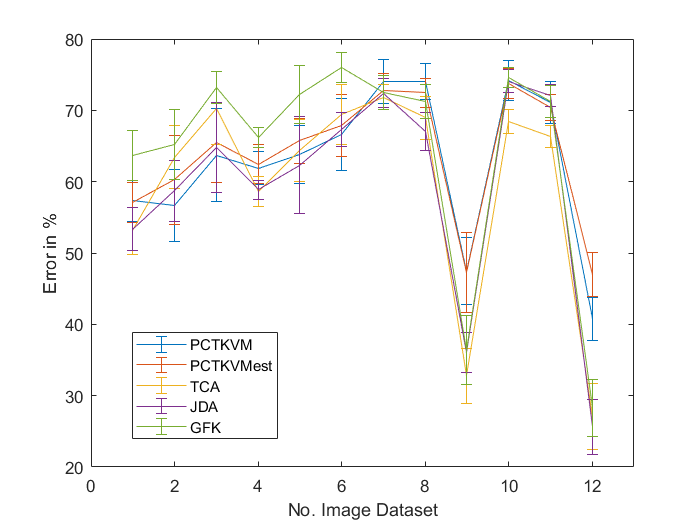
\includegraphics[width=1\linewidth]{figures/FiveTwoImageTL.png}
		\caption{\label{FigErrorImgTL}}
	\end{subfigure}%
	\begin{subfigure}{.5\textwidth}
		\centering
		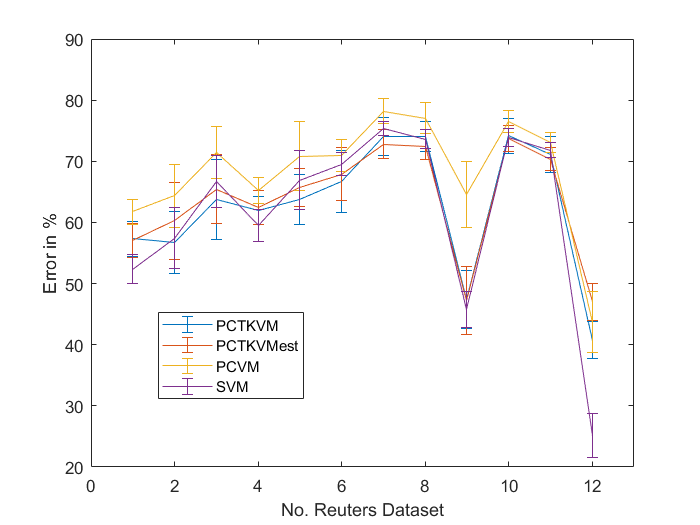
\includegraphics[width=1\linewidth]{figures/PerformanceImage.png}
		\caption{\label{FigErrorImgO}}
	\end{subfigure}
	\caption[Plot of mean Error and a standard Deviation on Image Dataset]{The plot of mean errors with standard deviation of the cross-validation. The left shows the transfer \acs{PCVM} in comparison with the other transfer learning solutions. The right side shows all \acs{PCVM}'s in comparison with \acs{SVM} and \acs{TKL}. A graph shows the error and a vertical bar shows the standard deviation. \label{FigErrorImgDatasetsB}}
\end{figure}

\begin{figure}[!]
	\centering
	\begin{subfigure}{.5\textwidth}
		\centering
		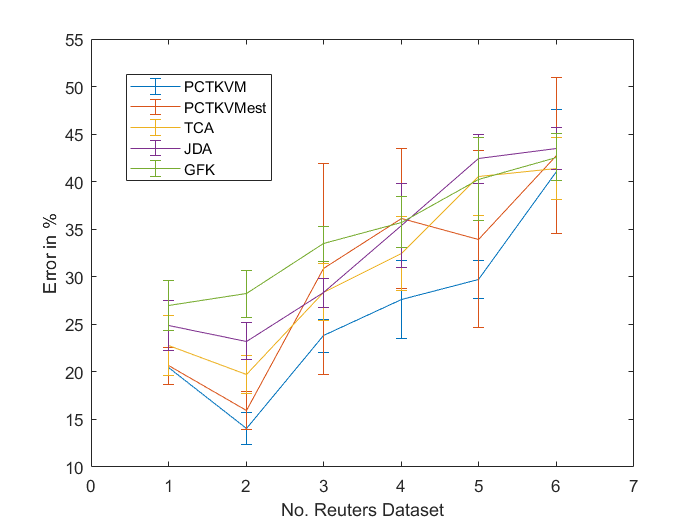
\includegraphics[width=1\linewidth]{figures/FiveTwoReutersTL.png}
		\caption{\label{FigErrorReuTL}}
	\end{subfigure}%
	\begin{subfigure}{.5\textwidth}
		\centering
		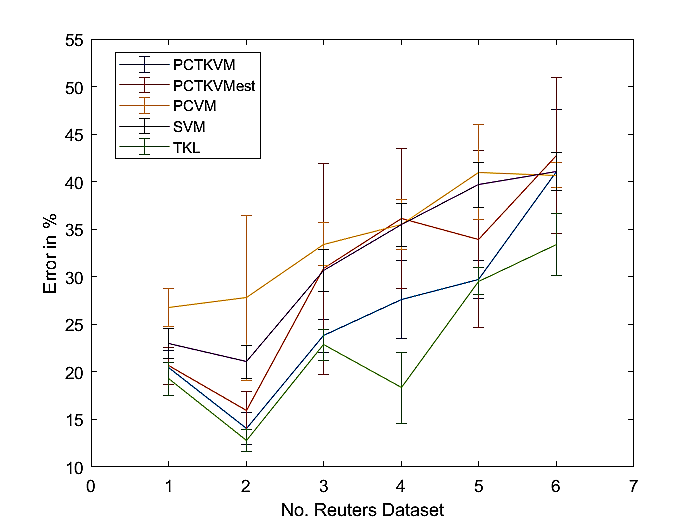
\includegraphics[width=1\linewidth]{figures/PerformanceReuters.png}
		\caption{\label{FigErrorReuO}}
	\end{subfigure}
	\caption[Plot of mean Error and standard Deviation on Reuters Dataset]{The plot of mean errors with standard deviation of the cross-validation. The left shows the transfer \acs{PCVM} in comparison with the other transfer learning solutions. The right side shows all \acs{PCVM}'s in comparison with \acs{SVM} and \acs{TKL}. A graph shows the error and a vertical bar shows the standard deviation. \label{FigErrorReutersDatasetsB}}
\end{figure}

\begin{table}[]
	\centering
	\resizebox{\textwidth}{!}{%
		\begin{tabular}{@{}ccccccccc@{}}
			\toprule
			\textbf{AUC Image}   & SVM   & PCVM  &  PCTKVM\textsubscript{$\theta$Est} & PCTKVM        & TCA   & JDA    & TKL            \\ \midrule
			C vs A               & 79.62 & 81.10 & 78.34 & 79.18          & 65.65 & 79.98 & 74.55 \\
			C vs D               & 64.36 & 89.85 & 95.12 & 96.98 & 58.86 & 72.98 		  & 68.76          \\
			C vs W               & 78.21 & 73.85 & 89.95 & 85.59          & 71.47 & 84.85 & 83.41 \\
			A vs C               & 74.93 & 73.48 & 74.31 & 72.29          & 66.36 & 71.37 & 69.78 \\
			A vs D               & 70.03 & 76.08 & 75.77 & 88.04 & 58.23 & 65.28 	      & 81.72          \\
			A vs W               & 77.70 & 73.40 & 81.35 & 82.82          & 66.82 & 72.82 & 80.80 \\
			D vs C               & 68.13 & 49.74 & 57.9 & 56.38          & 71.43 & 74.28 & 67.84 \\
			D vs A               & 76.25 & 35.30 & 45.64 & 45.02          & 79.09 & 78.97 & 77.51 \\
			D vs W               & 94.87 & 48.71 & 74.78 & 71.91          & 89.79 & 96.73 & 95.01 \\
			W vs C               & 58.39 & 56.29 & 56.08 & 57.20          & 62.92 & 70.04 & 63.22 \\
			W vs A               & 73.54 & 43.79 & 61.4 & 62.70          & 73.25 & 76.16 & 70.78 \\
			W vs D               & 72.48 & 89.56 & 93.61 & 97.21          & 73.36 & 79.56 & 92.26\\\midrule
			\textbf{AUC Reuters} & SVM   & PCVM  & PCTKVM\textsubscript{$\theta$Est} & PCTKVM      & TCA   & JDA   & TKL            \\\midrule
			Orgs vs People       & 81.14 & 80.29 & 88 & 88.62          & 83.45 & 80.34 & 90.43 \\
			People vs Orgs       & 82.23 & 81.08 & 91.48 & 92.64          & 85.98 & 82.39 & 93.61 \\
			Orgs vs Places       & 73.99 & 73.51 & 74.95 & 82.56          & 76.31 & 75.47 & 84.00 \\
			Places vs Orgs       & 69.50 & 69.97 & 77.35 & 80.21          & 72.86 & 68.59 & 89.50 \\
			Places vs People     & 59.36 & 63.11 & 71.77 & 77.15          & 60.95 & 58.72 & 76.57 \\
			People vs Places     & 47.77 & 57.78 & 55.25 & 54.97          & 54.35 & 49.15 & 66.63 \\ \bottomrule
	\end{tabular}}
	\caption[Complete Cross-Validtion Result of AUC]{Cross-validation comparison of the tested algorithms on 18 domain adaptation datasets by the AUC value. It shows the mean of the ten runs of cross-validation per dataset. The positive class is one, and the negative class is the composition of remaining classes.\label{BTableFTAUC}}
\end{table}


\begin{table}[]
	\centering
	\resizebox{\textwidth}{!}{%
		\begin{tabular}{@{}ccccccccc@{}}
			\toprule
			\textbf{N. SV. Image} & SVM    & PCVM   & PCTKVM\textsubscript{$\theta$Est} & PCTKVM & TCA    & JDA     & TKL    \\ \midrule
			C vs A                           & 556.70 & 125.80 & 87.6                               & 95.60  & 459.70 & 516.10 & 503.90 \\
			C vs D                           & 557.60 & 124.60 & 78.3                               & 87.80  & 466.80 & 522.20 & 522.30 \\
			C vs W                           & 557.30 & 126.40 & 82.2                               & 93.40  & 468.80 & 520.30 & 526.70 \\
			A vs C                           & 458.00 & 93.70  & 75.9                               & 79.20  & 356.30 & 416.70 & 412.30 \\
			A vs D                           & 455.80 & 92.70  & 62.4                               & 73.40  & 357.60 & 416.90 & 432.80 \\
			A vs W                           & 457.70 & 93.50  & 66.9                               & 76.70  & 357.00 & 416.10 & 429.30 \\
			D vs C                           & 78.50  & 20.50  & 18.7                               & 19.30  & 69.40  & 75.90  & 71.20  \\
			D vs A                           & 78.50  & 21.20  & 18.6                               & 18.90  & 69.30  & 76.00  & 72.60  \\
			D vs W                           & 78.50  & 20.80  & 19.2                               & 19.60  & 71.50  & 77.00  & 71.40  \\
			W vs C                           & 146.00 & 33.60  & 29.9                               & 31.70  & 119.70 & 137.00 & 127.90 \\
			W vs A                           & 146.70 & 33.90  & 29.5                               & 30.80  & 121.20 & 137.50 & 130.90 \\
			W vs D                           & 146.90 & 34.10  & 31                               & 32.10  & 122.30 & 137.50 & 126.70 \\ \midrule
			\textbf{N. SV. Reuters}        & SVM    & PCVM   & PCTKVM\textsubscript{$\theta$Est} & PCTKVM & TCA    & JDA    & TKL    \\ \midrule
			Orgs vs People                   & 514.60 & 33.80  & 2.7                               & 2.80   & 163.90 & 207.10 & 327.30 \\
			People vs Orgs                   & 526.20 & 54.10  & 2.6                               & 3.00   & 197.50 & 240.20 & 389.00 \\
			Orgs vs Places                   & 427.20 & 25.30  & 5.3                               & 3.10   & 155.50 & 187.20 & 355.00 \\
			Places vs Orgs                   & 464.00 & 30.10  & 2.2                               & 2.80   & 189.10 & 212.90 & 428.80 \\
			Places vs People                 & 477.70 & 58.30  & 2.9                               & 3.40   & 219.20 & 261.20 & 350.50 \\
			People vs Places                 & 484.40 & 80.00  & 2.4                               & 3.00   & 171.00 & 213.10 & 444.60 \\ \bottomrule
	\end{tabular}}
	\caption[Number of used support vectors from cross-validation]{A complete comparison of used support vectors in the cross-validation test over the 18 domain adaptation datasets. It shows the mean of the ten runs of cross-validation.\label{BTableFTNev}}
\end{table}
\begin{table}[]
	\centering
	\resizebox{\textwidth}{!}{%
		\begin{tabular}{@{}lllllllll@{}}
			\toprule
			\textbf{Time Image}   & SVM   & PCVM   & PCTKVM\textsubscript{$\theta$Est}& PCTKVM        & TCA   & JDA   & GFK   & TKL            \\ \midrule
			C vs A                & 0.11  & 468.91 & 33.19 & 35.10         & 1.95  & 1.37  & 0.71  & 0.78  \\
			C vs D                & 0.06  & 478.03 & 3.66 & 3.44 & 0.60  & 0.65  & 0.54  & 0.12           \\
			C vs W                & 0.07  & 490.87 & 6.03 & 6.87          & 0.74  & 0.74  & 0.56  & 0.16  \\
			A vs C                & 0.11  & 385.44 & 67.81 & 42.08         & 1.97  & 1.35  & 0.68  & 0.91  \\
			A vs D                & 0.04  & 385.38 & 4.59 & 4.37 & 0.41  & 0.51  & 0.46  & 0.07           \\
			A vs W                & 0.05  & 385.79 & 8.64 & 7.59          & 0.55  & 0.60  & 0.47  & 0.12  \\
			D vs C                & 0.04  & 68.15  & 25.94 & 26.44         & 0.55  & 0.61  & 0.40  & 0.71  \\
			D vs A                & 0.03  & 67.68  & 23.82 & 23.01         & 0.40  & 0.50  & 0.35  & 0.56  \\
			D vs W                & 0.01  & 69.87  & 5.14 & 5.54          & 0.06  & 0.13  & 0.21  & 0.07  \\
			W vs C                & 0.05  & 100.65 & 27.54 & 27.94         & 0.68  & 0.69  & 0.43  & 0.62  \\
			W vs A                & 0.04  & 102.59 & 29.39 & 26.62         & 0.51  & 0.58  & 0.38  & 0.43  \\
			W vs D                & 0.01  & 101.94 & 3.66 & 3.27          & 0.05  & 0.13  & 0.22  & 0.03  \\\midrule
			\textbf{Time Reuters} & SVM   & PCVM   & PCTKVM\textsubscript{$\theta$Est}& PCTKVM      & TCA   & JDA   & GFK   & TKL            \\\midrule
			Orgs vs People        & 15.59 & 694.52 & 15.32 & 20.35         & 20.95 & 24.13 & 44.65 & 15.82 \\
			People vs Orgs        & 14.66 & 656.70 & 15.61 & 20.29         & 21.08 & 24.72 & 43.79 & 15.69 \\
			Orgs vs Places        & 9.93  & 451.34 & 11.03 & 13.37         & 14.10 & 16.00 & 34.36 & 10.71 \\
			Places vs Orgs        & 10.20 & 474.43 & 11.3 & 14.87         & 13.72 & 15.72 & 35.77 & 10.88 \\
			Places vs People      & 11.55 & 525.75 & 11.92 & 15.46         & 15.23 & 17.39 & 39.16 & 11.98 \\
			People vs Places      & 9.27  & 459.54 & 11.48 & 12.83         & 12.31 & 14.82 & 22.30 & 9.67  \\ \bottomrule
	\end{tabular}}
	\caption[Time comparison from cross-validation]{Comparison of the absolute running time in seconds in the cross-validation test over the 18 datasets. It shows the mean time of the ten runs of cross-validation\label{BTableFTTime}}
\end{table}
\section{Complete Dataset Comparison}\label{BSecCom}
This section shows the results of the classifiers trained on the whole dataset. 
In general, the tables are showing the mean over five runs and are separated in the Reuters and image dataset.
In table \ref{BTableCompleteErr} are the error and \acs{RMSE} values shown.
This results are also plotted in figure \ref{FigErrorImgDatasetsB} for images and plotted in figure \ref{FigErrorReutersDatasetsB} for Reuters.
The numbers of a dataset is the order of the sets, shown for example in \ref{BTableFTErr}.
The \acs{AUC} values are shown in table \ref{BTableCompletAUC}.
For a complete overview over the used support vectors, see table \ref{BTableCompleteNvec}.
Finally, the computation time in second as the mean over five runs is shown in \ref{BTableCompleteTime}. 
\begin{table}[h]
	\centering
	\resizebox{\textwidth}{!}{%
		\begin{tabular}{@{}ccccccccc@{}}
			\toprule
			\textbf{Error Image}   & SVM   & PCVM  & PCTKVM\textsubscript{$\theta$Est}& PCTKVM         & TCA   & JDA   & GFK   & TKL            \\ \midrule
			C vs A                 & 46.66 & 55.80(1.06) & 50.71 (2.18)  & 46.26  (1.75)        & 44.89 & 42.17 & 59.92 & 44.05 \\
			C vs D                 & 51.59 & 64.97 (2.25)& 50.83 (4.51)  & 50.83 (4.06)& 54.14 & 56.69 & 58.60 & 54.78          \\
			C vs W                 & 59.32 & 66.31 (2.73)& 55.05 (3.95)  & 51.93  (2.48)        & 54.58 & 51.19 & 64.41 & 49.15 \\
			A vs C                 & 56.10 & 62.85 (1.62)& 56.81 (0.21)  & 55.10  (0.69)        & 54.23 & 54.59 & 59.75 & 54.05 \\
			A vs D                 & 54.78 & 68.15 (4.18)& 60    (2.6)  & 52.61 (3.17)& 62.42 & 65.61 & 61.78 & 52.87          \\
			A vs W                 & 61.69 & 71.12 (2.01)& 64.2  (3.22)  & 58.51  (1.55)        & 60.68 & 55.93 & 62.03 & 57.29 \\
			D vs C                 & 70.44 & 73.00 (1.3)&  67.14 (0.41) & 66.45  (1.11)        & 63.05 & 65.63 & 71.42 & 61.00 \\
			D vs A                 & 69.83 & 72.11 (1.63)& 66.12 (0.75)  & 63.82  (1.30)        & 61.59 & 62.63 & 66.39 & 60.96 \\
			D vs W                 & 37.63 & 60.20 (4.96)& 29.83 (3.12)  & 29.08   (3.99)       & 14.58 & 15.59 & 17.29 & 13.90 \\
			W vs C                 & 74.35 & 72.45 (0.84)& 67.16 (0.7)  & 67.03   (1.09)       & 67.94 & 68.12 & 71.15 & 65.00 \\
			W vs A                 & 67.85 & 71.84 (1.4)& 64.86  (1.87)& 64.61   (1.84)       & 64.41 & 66.81 & 66.91 & 62.00 \\
			W vs D                 & 15.29 & 37.71 (3.03)& 33.12 (1.49)  & 26.75   (1.01)       & 15.92 & 11.46 & 11.46 & 15.29 \\\midrule
			RSME                   & 55.46 & 64.71 (10.1) & 55.80(12.28)     & 52.75 (13.4)         & 51.53 & 51.37 & 55.93 & 49.19 \\\midrule
			\textbf{Error Reuters} & SVM   & PCVM  & PCTKVM\textsubscript{$\theta$Est}& PCTKVM       & TCA   & JDA   & GFK   & TKL            \\\midrule
			Orgs vs People         & 23.26 & 30.17(6)   &  19.97 (1.42)	    & 19.72  (0.86)        & 22.93 & 24.83 & 25.33 & 18.05 \\
			People vs Orgs         & 21.75 & 25.16(2.83) & 19.97 (1.42)	    & 13.76 (0.38)         & 20.45 & 24.17 & 27.49 & 12.29 \\
			Orgs vs Places         & 30.01 & 36.82 (5.24)& 33.27 (15.92)    & 24.20  (0.62)        & 28.19 & 27.04 & 32.69 & 23.20 \\
			Places vs Orgs         & 37.01 & 37.48 (2.34)& 33.27 (15.92)    & 33.94  (9.65)        & 30.31 & 34.65 & 37.70 & 16.73 \\
			Places vs People       & 39.28 & 41.30 (1.97)& 43.03 (14.37)    & 29.38   (0.33)       & 41.04 & 43.73 & 42.62 & 29.71 \\
			People vs Places       & 41.60 & 41.54 (0.90)& 43.03 (14.37)    & 39.74    (0)      & 47.08 & 44.57 & 43.64 & 33.05 \\\midrule
			RSME                   & 32.15 & 35.41(6.5) & 34.09 (8.0)    & 26.79 (9.67)         & 31.67 & 33.16 & 34.91 & 22.17 \\ \bottomrule
	\end{tabular}}
	\caption[Complete Dataset Result of Error]{The test result of the classifiers by using the whole 18 datasets. It shows the mean error over five runs.\label{BTableCompleteErr}}
\end{table}

\begin{figure}[!]
	\centering
	\begin{subfigure}{.5\textwidth}
		\centering
		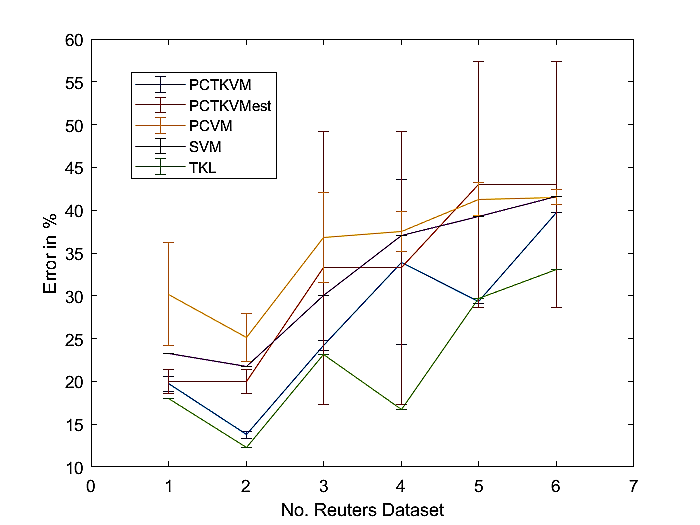
\includegraphics[width=1\linewidth]{figures/AverageReuters.png}
		\caption{\label{FigErrorAvReuTL}}
	\end{subfigure}%
	\begin{subfigure}{.5\textwidth}
		\centering
		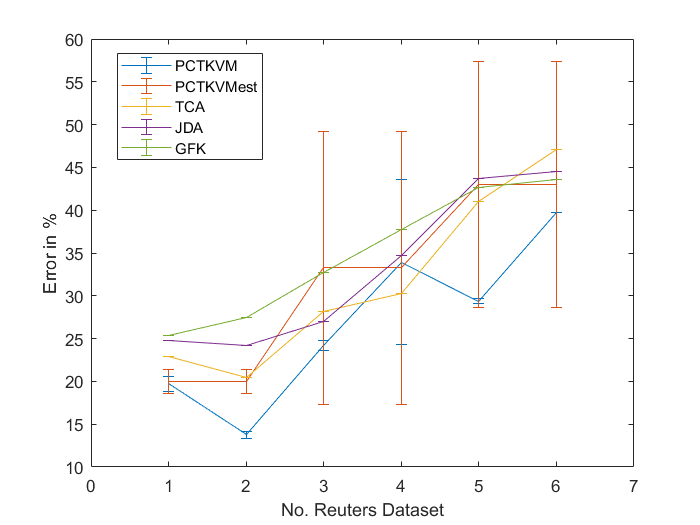
\includegraphics[width=1\linewidth]{figures/AverageReutersTL.png}
		\caption{\label{FigErrorAvReuO}}
	\end{subfigure}
	\begin{subfigure}{.5\textwidth}
		\centering
		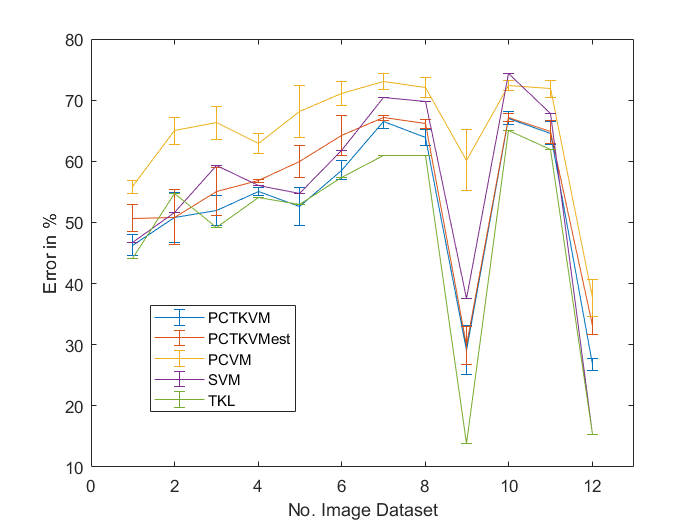
\includegraphics[width=1\linewidth]{figures/AverageImage.png}
		\caption{\label{FigErrorAvImTL}}
	\end{subfigure}%
	\begin{subfigure}{.5\textwidth}
		\centering
		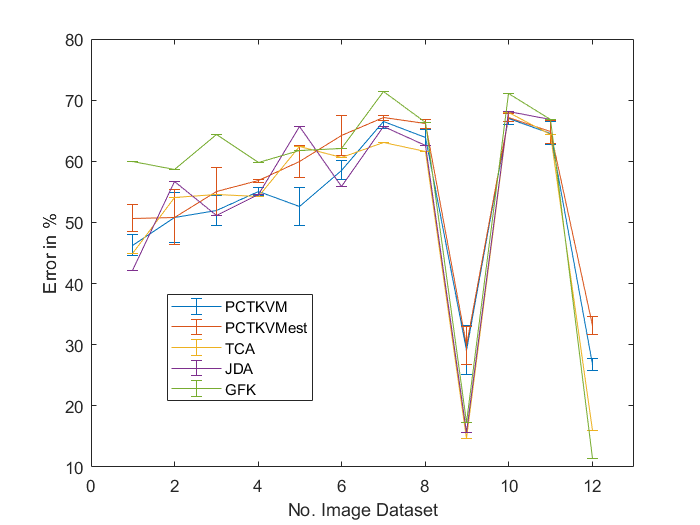
\includegraphics[width=1\linewidth]{figures/AverageImageTL.png}
		\caption{\label{FigErrorAvImO}}
	\end{subfigure}
	\caption[Plot of mean Error and standard Deviation on the whole Datasets]{The plot of mean errors with a standard deviation on the whole datasets. The left side shows all \acs{PCVM}'s in comparison with \acs{SVM} and \acs{TKL}. The right side shows all \acs{PCVM}'s in comparison to the other transfer learning solutions. The first row shows the result on Reuters and the second row illustrates the result on image dataset. A graph shows the error and a vertical bar shows the standard deviation. \label{FigErrorAv}}
\end{figure}


\begin{table}[]
	\centering
	\resizebox{\textwidth}{!}{%
		\begin{tabular}{@{}ccccccccc@{}}
			\toprule
			\textbf{AUC Image}   & SVM   & PCVM  & PCTKVM\textsubscript{$\theta$Est} & PCTKVM      & TCA   & JDA   & TKL            \\ \midrule
			C vs A               & 71.75 & 85.73 & 84.53     & 85.81          & 64.21 & 71.67 & 65.76 \\
			C vs D               & 56.78 & 94.85 & 93.37     & 90.78 & 60.40 & 68.45 		  & 51.49          \\
			C vs W               & 67.15 & 85.61 & 90.15     & 95.74          & 50.75 & 64.92 & 78.47 \\
			A vs C               & 74.87 & 73.38 & 78.09     & 76.09          & 58.27 & 73.57 & 74.39 \\
			A vs D               & 72.93 & 78.89 & 97.26     & 88.37 & 57.53 & 71.84 		  & 78.68          \\
			A vs W               & 86.48 & 68.09 & 86.57     & 80.38          & 77.50 & 75.36 & 82.81 \\
			D vs C               & 76.33 & 52.52 & 61.55     & 50.66          & 82.63 & 80.23 & 78.78 \\
			D vs A               & 79.78 & 54.52 & 66.8    & 52.47          & 85.83 & 86.81 & 82.57 \\
			D vs W               & 96.36 & 52.31 & 73.54     & 70.18          & 76.33 & 98.03 & 97.24 \\
			W vs C               & 66.91 & 54.76 & 69.74     & 66.82          & 70.11 & 77.41 & 71.79 \\
			W vs A               & 72.46 & 49.93 & 62.46     & 64.64          & 74.36 & 84.21 & 77.75 \\
			W vs D               & 80.69 & 84.91 & 93.05     & 98.70          & 84.02 & 90.29 & 93.28 \\\midrule
			\textbf{AUC Reuters} & SVM   & PCVM  & PCTKVM\textsubscript{$\theta$Est} & PCTKVM      & TCA   & JDA    & TKL            \\\midrule
			Orgs vs People       & 79.97 & 79.00 & 89     & 89.54          & 83.80 & 81.13  & 90.70 \\
			People vs Orgs       & 80.35 & 81.60 & 89     & 92.57          & 84.27 & 81.95  & 93.69 \\
			Orgs vs Places       & 72.83 & 70.96 & 74.47     & 83.55          & 77.08 & 76.46  & 84.79 \\
			Places vs Orgs       & 66.40 & 69.89 & 74.47     & 87.33          & 74.64 & 69.55  & 91.34 \\
			Places vs People     & 56.36 & 60.64 & 66.2     & 77.03          & 56.78 & 56.43  & 76.31 \\
			People vs Places     & 42.59 & 51.82 & 66.2     & 58.40          & 39.85 & 45.87  & 66.95 \\ \bottomrule
	\end{tabular}}
	\caption[Complete Dataset Result of AUC]{The test result of the classifiers by using the whole 18 datasets. It shows the mean AUC value over five runs. The positive class is one, and the negative class is the composition of remaining classes.\label{BTableCompletAUC}}
\end{table}

\begin{table}[]
	\centering
	\resizebox{\textwidth}{!}{%
		\begin{tabular}{@{}ccccccccc@{}}
			\toprule
			\textbf{N. SV. Image} & SVM     & PCVM   & PCTKVM\textsubscript{$\theta$Est} & PCTKVM & TCA    & JDA   & TKL    \\ \midrule
			C vs A                           & 1098.00 & 242.80 & 109.8                                   & 153.00 & 818.00 & 973.00 & 937.00 \\
			C vs D                           & 1098.00 & 257.20 & 105.8                                   & 130.60 & 828.00 & 976.00 & 983.00 \\
			C vs W                           & 1098.00 & 246.20 & 116.2                                   & 137.00 & 834.00 & 980.00 & 976.50 \\
			A vs C                           & 898.00  & 187.40 & 113                                   & 128.80 & 577.00 & 726.00 & 749.00 \\
			A vs D                           & 898.00  & 184.00 & 93                                   & 114.60 & 581.00 & 729.00 & 829.00 \\
			A vs W                           & 898.00  & 188.40 & 101.6                                   & 112.60 & 588.00 & 742.00 & 791.00 \\
			D vs C                           & 157.00  & 39.80  & 35.6                                   & 37.60  & 130.00 & 149.00 & 137.00 \\
			D vs A                           & 157.00  & 37.20  & 32.8                                   & 35.00  & 134.00 & 149.00 & 139.00 \\
			D vs W                           & 157.00  & 41.40  & 33                                   & 36.00  & 138.00 & 149.00 & 130.00 \\
			W vs C                           & 295.00  & 65.20  & 55                                   & 53.80  & 214.00 & 273.00 & 248.00 \\
			W vs A                           & 295.00  & 64.00  & 51.4                                   & 53.80  & 210.00 & 270.00 & 248.00 \\
			W vs D                           & 295.00  & 63.40  & 53.4                                   & 55.20  & 224.00 & 275.00 & 239.00 \\ \midrule
			\textbf{N. SV. Reuters}        & SVM     & PCVM   & PCTKVM\textsubscript{$\theta$Est} & PCTKVM & TCA    & JDA   & TKL    \\ \midrule
			Orgs vs People                   & 850.00  & 66.60  & 3                                  & 2.40   & 280.00 & 329.00 & 604.00 \\
			People vs Orgs                   & 867.50  & 53.60  & 3                                  & 2.80   & 309.00 & 356.50 & 667.00 \\
			Orgs vs Places                   & 708.00  & 60.80  & 2                                  & 2.80   & 265.00 & 274.00 & 679.00 \\
			Places vs Orgs                   & 752.00  & 43.00  & 2                                  & 3.00   & 291.50 & 297.00 & 746.50 \\
			Places vs People                 & 845.00  & 48.00  & 4                                  & 4.00   & 362.00 & 447.00 & 659.00 \\
			People vs Places                 & 838.50  & 54.00  & 4                                  & 2.20   & 315.50 & 390.50 & 748.50 \\ \bottomrule
	\end{tabular}}
	\caption[Complete number of used support vectors]{Comparison of the number of used support vectors for the whole 18 datasets. It shows the mean number over five runs.\label{BTableCompleteNvec}}
\end{table}

\begin{table}[]
	\centering
	\resizebox{\textwidth}{!}{%
		\begin{tabular}{@{}ccccccccc@{}}
			\toprule
			\textbf{Time Image}   & SVM   & PCVM    &PCTKVM\textsubscript{$\theta$Est}& PCTKVM      & TCA   & JDA    & GFK   & TKL            \\ \midrule
			C vs A                & 0.41  & 1561.72 & 124.38     & 95.19          & 12.72 & 5.66   & 1.58  & 1.70  \\
			C vs D                & 0.19  & 1534.87 & 13.51     & 10.20 & 3.85  & 2.21   & 1.04  & 0.28           \\
			C vs W                & 0.22  & 1523.58 & 17.97     & 39.27          & 4.58  & 2.61   & 1.10  & 0.71  \\
			A vs C                & 0.36  & 1167.97 & 133.97     & 77.53          & 12.07 & 5.51   & 1.53  & 2.01  \\
			A vs D                & 0.14  & 1188.29 & 11.61     & 9.76  & 2.55  & 1.76   & 0.97  & 0.22           \\
			A vs W                & 0.16  & 1175.60 & 17.16     & 63.73          & 3.27  & 2.09   & 1.00  & 0.61  \\
			D vs C                & 0.12  & 104.43  & 80.73     & 70.93          & 3.31  & 2.09   & 0.81  & 1.43  \\
			D vs A                & 0.10  & 106.09  & 72.52     & 50.58          & 2.27  & 1.68   & 0.72  & 1.04  \\
			D vs W                & 0.02  & 106.48  & 14.7     & 14.68          & 0.24  & 0.36   & 0.29  & 0.43  \\
			W vs C                & 0.15  & 179.01  & 81.85     & 92.44          & 4.30  & 2.62   & 0.93  & 1.65  \\
			W vs A                & 0.12  & 177.99  & 66.65     & 62.21          & 3.12  & 2.03   & 0.78  & 1.12  \\
			W vs D                & 0.02  & 177.49  & 10.66     & 8.14           & 0.26  & 0.37   & 0.32  & 0.11  \\\midrule
			\textbf{Time Reuters} & SVM   & PCVM    & PCTKVM\textsubscript{$\theta$Est} & PCTKVM        & TCA   & JDA    & GFK   & TKL            \\\midrule
			Orgs vs People        & 49.48 & 2256.50 & 64.23    & 61.25          & 73.74 & 103.73 & 33.24 & 49.19 \\
			People vs Orgs        & 47.16 & 2024.11 & 64.23    & 67.62          & 69.82 & 100.04 & 32.68 & 47.86 \\
			Orgs vs Places        & 34.79 & 1529.51 & 45.37    & 47.62          & 51.44 & 69.37  & 27.66 & 34.53 \\
			Places vs Orgs        & 33.18 & 1488.56 & 45.37    & 52.41          & 46.38 & 66.13  & 27.28 & 36.25 \\
			Places vs People      & 38.01 & 1794.56 & 51.49    & 56.30          & 63.67 & 88.54  & 30.87 & 43.54 \\
			People vs Places      & 37.11 & 1641.59 & 51.49    & 60.23          & 53.68 & 77.32  & 28.37 & 38.70 \\ \bottomrule
	\end{tabular}}
	\caption[Time comparison of whole dataset]{Comparison of the absolute running time in second for the whole 18 datasets as mean. It shows the mean time of five runs.\label{BTableCompleteTime}}
\end{table}
